% Options for packages loaded elsewhere
\PassOptionsToPackage{unicode}{hyperref}
\PassOptionsToPackage{hyphens}{url}
\PassOptionsToPackage{dvipsnames,svgnames,x11names}{xcolor}
%
\documentclass[
  letterpaper,
  DIV=11,
  numbers=noendperiod]{scrartcl}

\usepackage{amsmath,amssymb}
\usepackage{iftex}
\ifPDFTeX
  \usepackage[T1]{fontenc}
  \usepackage[utf8]{inputenc}
  \usepackage{textcomp} % provide euro and other symbols
\else % if luatex or xetex
  \usepackage{unicode-math}
  \defaultfontfeatures{Scale=MatchLowercase}
  \defaultfontfeatures[\rmfamily]{Ligatures=TeX,Scale=1}
\fi
\usepackage{lmodern}
\ifPDFTeX\else  
    % xetex/luatex font selection
\fi
% Use upquote if available, for straight quotes in verbatim environments
\IfFileExists{upquote.sty}{\usepackage{upquote}}{}
\IfFileExists{microtype.sty}{% use microtype if available
  \usepackage[]{microtype}
  \UseMicrotypeSet[protrusion]{basicmath} % disable protrusion for tt fonts
}{}
\makeatletter
\@ifundefined{KOMAClassName}{% if non-KOMA class
  \IfFileExists{parskip.sty}{%
    \usepackage{parskip}
  }{% else
    \setlength{\parindent}{0pt}
    \setlength{\parskip}{6pt plus 2pt minus 1pt}}
}{% if KOMA class
  \KOMAoptions{parskip=half}}
\makeatother
\usepackage{xcolor}
\ifLuaTeX
  \usepackage{luacolor}
  \usepackage[soul]{lua-ul}
\else
  \usepackage{soul}
  
\fi
\setlength{\emergencystretch}{3em} % prevent overfull lines
\setcounter{secnumdepth}{-\maxdimen} % remove section numbering
% Make \paragraph and \subparagraph free-standing
\ifx\paragraph\undefined\else
  \let\oldparagraph\paragraph
  \renewcommand{\paragraph}[1]{\oldparagraph{#1}\mbox{}}
\fi
\ifx\subparagraph\undefined\else
  \let\oldsubparagraph\subparagraph
  \renewcommand{\subparagraph}[1]{\oldsubparagraph{#1}\mbox{}}
\fi


\providecommand{\tightlist}{%
  \setlength{\itemsep}{0pt}\setlength{\parskip}{0pt}}\usepackage{longtable,booktabs,array}
\usepackage{calc} % for calculating minipage widths
% Correct order of tables after \paragraph or \subparagraph
\usepackage{etoolbox}
\makeatletter
\patchcmd\longtable{\par}{\if@noskipsec\mbox{}\fi\par}{}{}
\makeatother
% Allow footnotes in longtable head/foot
\IfFileExists{footnotehyper.sty}{\usepackage{footnotehyper}}{\usepackage{footnote}}
\makesavenoteenv{longtable}
\usepackage{graphicx}
\makeatletter
\def\maxwidth{\ifdim\Gin@nat@width>\linewidth\linewidth\else\Gin@nat@width\fi}
\def\maxheight{\ifdim\Gin@nat@height>\textheight\textheight\else\Gin@nat@height\fi}
\makeatother
% Scale images if necessary, so that they will not overflow the page
% margins by default, and it is still possible to overwrite the defaults
% using explicit options in \includegraphics[width, height, ...]{}
\setkeys{Gin}{width=\maxwidth,height=\maxheight,keepaspectratio}
% Set default figure placement to htbp
\makeatletter
\def\fps@figure{htbp}
\makeatother

\KOMAoption{captions}{tableheading}
\makeatletter
\@ifpackageloaded{caption}{}{\usepackage{caption}}
\AtBeginDocument{%
\ifdefined\contentsname
  \renewcommand*\contentsname{Table of contents}
\else
  \newcommand\contentsname{Table of contents}
\fi
\ifdefined\listfigurename
  \renewcommand*\listfigurename{List of Figures}
\else
  \newcommand\listfigurename{List of Figures}
\fi
\ifdefined\listtablename
  \renewcommand*\listtablename{List of Tables}
\else
  \newcommand\listtablename{List of Tables}
\fi
\ifdefined\figurename
  \renewcommand*\figurename{Figure}
\else
  \newcommand\figurename{Figure}
\fi
\ifdefined\tablename
  \renewcommand*\tablename{Table}
\else
  \newcommand\tablename{Table}
\fi
}
\@ifpackageloaded{float}{}{\usepackage{float}}
\floatstyle{ruled}
\@ifundefined{c@chapter}{\newfloat{codelisting}{h}{lop}}{\newfloat{codelisting}{h}{lop}[chapter]}
\floatname{codelisting}{Listing}
\newcommand*\listoflistings{\listof{codelisting}{List of Listings}}
\makeatother
\makeatletter
\makeatother
\makeatletter
\@ifpackageloaded{caption}{}{\usepackage{caption}}
\@ifpackageloaded{subcaption}{}{\usepackage{subcaption}}
\makeatother
\ifLuaTeX
  \usepackage{selnolig}  % disable illegal ligatures
\fi
\usepackage{bookmark}

\IfFileExists{xurl.sty}{\usepackage{xurl}}{} % add URL line breaks if available
\urlstyle{same} % disable monospaced font for URLs
\hypersetup{
  pdftitle={Econometric Approach},
  pdfauthor={Lennart Joop and Julia Daetz},
  colorlinks=true,
  linkcolor={blue},
  filecolor={Maroon},
  citecolor={Blue},
  urlcolor={Blue},
  pdfcreator={LaTeX via pandoc}}

\title{Econometric Approach}
\author{Lennart Joop and Julia Daetz}
\date{}

\begin{document}
\maketitle

This document presents the econometric approach we used in our research
project, as described in Milestone 3.

\subsection{Economic Model}\label{economic-model}

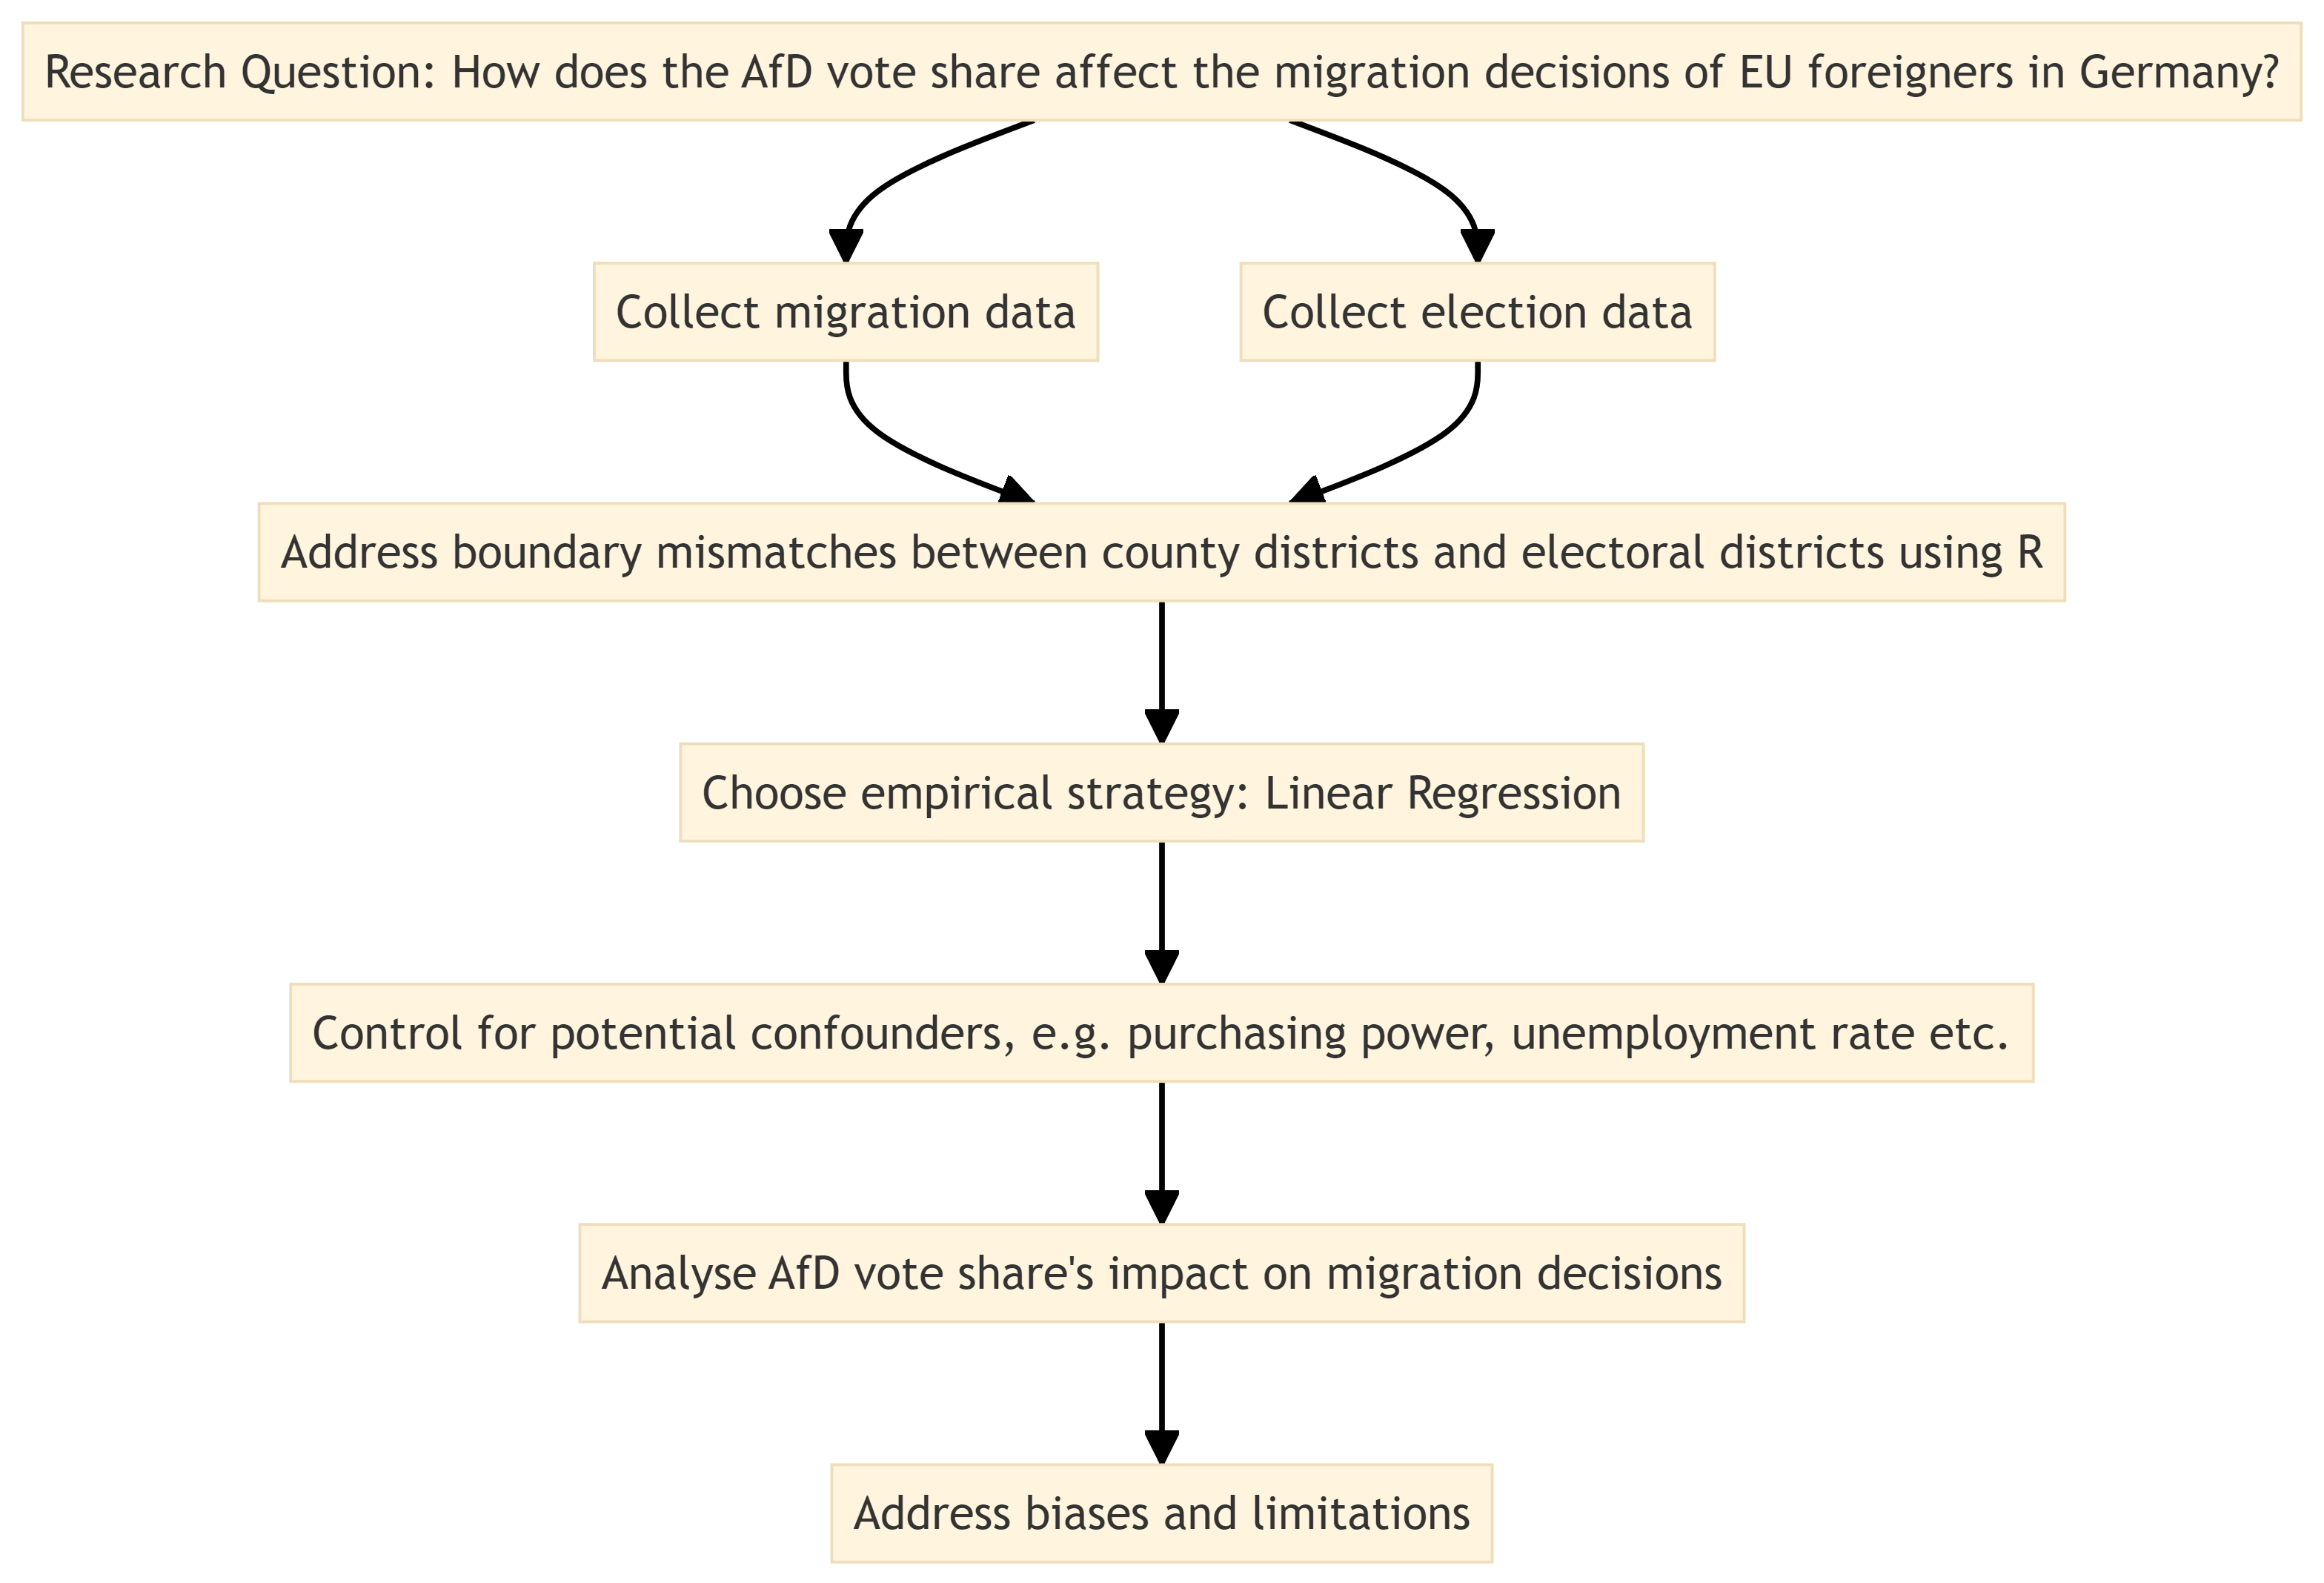
\includegraphics[width=8.46in,height=5.77in]{Econometric_Approach_files/figure-latex/mermaid-figure-1.png}

Flow Chart Empirical Strategy

\subsection{Setting}\label{setting}

\textbf{Endogenous Variable:} Xenophobia which we proxy by using AfD
election results

\textbf{Main Outcome Variable:} The percentage change of the number of
EU migrants

Our observation units are 299 German voting districts. We run four
different regressions in four years. We want to find the impact of AfD
vote share in the elections 2017 and 2021 on the change of EU migrants 3
months and 15 months after the election.

Because AfD vote shares are non-binary, we observe a treatment intensity
instead of a treatment effect. Each unit of observation has a different
treatment intensity which is based on the AfD vote shares.

\subsection{Mechanism}\label{mechanism}

Due to our analysis being a simple regression, it is possible to test
direct relationships between endogenous and main outcome variable. We
plan on running simple regressions that just show the relation between
our two main variables, reverse regressions to test for reverse
causalities and simple regressions between our control variables and the
main outcome variable.

\subsection{Sources of Bias and
Identification}\label{sources-of-bias-and-identification}

The connection we are trying to evaluate is hard to isolate cleanly. To
isolate the effect of AfD vote shares we introduce control variables
aiming to capture the influence of potential confounders. Based on our
general intuition and the above introduced underlying studies, which
highlight the impact of economic, social, and other factors on
foreigners decisions to migrate, we employ the following six control
variables. Even though the mentioned studies focus on the conditions in
peoples home countries \emph{before} the migration process (or even the
decision making process), it seems intuitive that similar variables,
e.g.~economic outlook, social networks etc., might also have an effect
on the destination choices of migrants, when looking at potential
destination countries.

The control variable ``Big Cities'' is supposed to capture the impact of
greater attractiveness of large cities due to better economic
opportunities, better access to healthcare and other social factors.

The control variable ``East Germany'' is supposed to capture the impact
of the differences between East and West Germany such as political
climate, mentality and economic opportunities.

The control variable ``Total amount of migrants'' is supposed to capture
the impact of the attractiveness of a region due to an already existing
population of migrants which helps with integration and the access to a
social group of people of similar culture.

The control variable ``Unemployment'' and ``Purchase Power'' are
supposed to capture the impact of economic influences on migration
decisions.

The control variable ``Healthcare'' is supposed to capture impact of
access to healthcare on migration decisions.

We assume the overall direction of this bias is positive. Despite
including several factors that could influence migration decisions there
are still many factors that still could influence such a complex choice.
We have an omitted variable bias. We are not able to include all of them
in our model. This leads to an overestimation of the effect of AfD
voting results on the change of EU migrants.

Another source of potential bias is the creation of our data set. We
assign our federal district data to the voting districts by weighting
the data via the share of area of the federal district that is in the
voting district. This is just an approximation and differs from the real
distribution of the population and migrants. Unfortunately, we have no
way of removing or isolating this bias.We also don't know the direction
of this bias. It could be positive if the data shows that voting
districts with the highest AfD voting results occupy a larger share of
the federal district area while actually having a smaller population.
However, the reverse could also be true.

\textbf{Formulas}

\ul{baseline OLS formulas:}

\emph{\texttt{main\ outcome\ variable\ \textless{}-\ endogenous\ variable}}

\ul{with the following pairings:}

\textbf{1)}\\
MOV: Percentage change of EU migrants 31.12.2017 compared to 31.12.2016

EV: Vote results of the AFD on 24.09.2017

\textbf{2)}\\
MOV: Percentage change of EU migrants 31.12.2018 compared to 31.12.2016

EV: Vote results of the AFD on 24.09.2017

\textbf{3)}\\
MOV: Percentage change of EU migrants 31.12.2021 compared to 31.12.2020

EV: Vote results of the AFD on 26.09.2021

\textbf{4)}\\
MOV: Percentage change of EU migrants 31.12.2022 compared to 31.12.2020

EV: Vote results of the AFD on 26.09.2021

\ul{OLS formula with control variables:}

\texttt{main\ outcome\ variable\ \textless{}-\ endogenous\ variable\ +\ control\ variables}

\ul{with the following pairings:}

\textbf{1)}\\
MOV: Percentage change of EU migrants 31.12.2017 compared to 31.12.2016

EV: Vote results of the AFD on 24.09.2017

CV:

\begin{itemize}
\item
  Dummy variable Big Cities (time indifferent)
\item
  Dummy variable East Germany (time indifferent)
\item
  Total amount of migrants on 31.12.2016
\item
  Unemployment rate on 31.12.2017
\item
  Average purchasing power on 31.12.2017
\item
  Access to hospital beds per 1000 inhabitants on 31.12.2017
\end{itemize}

\textbf{2)}\\
MOV: Percentage change of EU migrants 31.12.2018 compared to 31.12.2016

EV: Vote results of the AFD on 24.09.2017

CV:

\begin{itemize}
\item
  Dummy variable Big Cities (time indifferent)
\item
  Dummy variable East Germany (time indifferent)
\item
  Total amount of migrants on 31.12.2017
\item
  Unemployment rate on 31.12.2018
\item
  Average purchasing power on 31.12.2018
\item
  Access to hospital beds per 1000 inhabitants on 31.12.2018
\end{itemize}

\textbf{3)}\\
MOV: Percentage change of EU migrants 31.12.2021 compared to 31.12.2020

EV: Vote results of the AFD on 26.09.2021

CV:

\begin{itemize}
\item
  Dummy variable Big Cities (time indifferent)
\item
  Dummy variable East Germany (time indifferent)
\item
  Total amount of migrants on 31.12.2020
\item
  Unemployment rate on 31.12.2021
\item
  Average purchasing power on 31.12.2021
\item
  Access to hospital beds per 1000 inhabitants on 31.12.2021
\end{itemize}

\textbf{4)}\\
MOV: Percentage change of EU migrants 31.12.2022 compared to 31.12.2020

EV: Vote results of the AFD on 26.09.2021

CV:

\begin{itemize}
\item
  Dummy variable Big Cities (time indifferent)
\item
  Dummy variable East Germany (time indifferent)
\item
  Total amount of migrants on 31.12.2020
\item
  Unemployment rate on 31.12.2021
\item
  Average purchasing power on 31.12.2021
\item
  Access to hospital beds per 1000 inhabitants on 31.12.2021
\end{itemize}

\subsection{Treatment}\label{treatment}

We want to identify an effect of vote shares of the AfD on the migration
decisions of EU foreigners in Germany. We assume that voting districts,
which have a higher share of AfD voters, are more xenophobic. This
xenophobia could lead to a decrease in the number of EU migrants in the
following years. This decrease could either be motivated passively:
higher AfD vote shares indicates higher xenophobia which decreases the
live quality of EU foreigners, or actively: EU migrants inform
themselves about the elections and choose not to live in regions with
high shares of AfD voters.



\end{document}
